\documentclass{ximera}

\newcommand{\RR}{\mathbb R}
\renewcommand{\d}{\,d}
\newcommand{\dd}[2][]{\frac{d #1}{d #2}}
\renewcommand{\l}{\ell}
\newcommand{\ddx}{\frac{d}{dx}}
\newcommand{\dfn}{\textbf}
\newcommand{\eval}[1]{\bigg[ #1 \bigg]}



\outcome{Use Pythagorean identities to simplify expressions.}
\outcome{Substitute trigonometric functions to simiplify integrals.}
\outcome{Complete the square to change the form of an integral.}

\title[Dig-In:]{Trigonometric substitution}

\begin{document}
\begin{abstract}
  We integrate by substitution with the appropriate trigonometric
  function.
\end{abstract}
\maketitle

One useful model of the definite integral is that of a ``machine''
that computes ``signed area under the curve.'' In particular, this
metaphor allows us to compute
\[
\int_{-1}^1 \sqrt{1-x^2} \d x
\]
via geometry. Check out a graph of $y= \sqrt{1-x^2}$:
\begin{image}
  \begin{tikzpicture}
    \begin{axis}[
        width=6in,
        %height=3in,
        unit vector ratio*=1 1 1,            
        xmin=-1.1, xmax=1.1,ymin=-.1,ymax=1.1,
        axis lines =center, xlabel=$x$, ylabel=$y$,
        every axis y label/.style={at=(current axis.above origin),anchor=south},
        every axis x label/.style={at=(current axis.right of origin),anchor=west},
        axis on top,
      ] 
      \addplot [draw=none, fill=fillp,samples=200,domain=-1:1] {sqrt(1-x^2)} \closedcycle;
      
      \addplot [penColor,very thick,samples=200,domain=-1:1] {sqrt(1-x^2)};
    \end{axis}
  \end{tikzpicture}
\end{image}

\begin{question}
  Using the graph above and basic facts from geometry, compute:
  \[
  \int_{-1}^1 \sqrt{1-x^2} \d x = \answer{\pi/2}
  \]
\end{question}

We now know a number of integration techniques, yet we are still
unable to evaluate the above integral without resorting to a geometric
interpretation!  This section introduces \dfn{trigonometric substitution},
a method of integration that will give us a new tool in our quest to compute all integrals.
This technique works on the same principle as substitution. Recall the
substitution formula, rewritten with suggestive notation:

\begin{theorem}[Integral Substitution Formula]\index{substitution formula}  
If a function $x$ is differentiable on the interval $[a,b]$, then
\[
\int_{x(a)}^{x(b)} f(x) \d x = \int_a^b f(x(\theta)) x'(\theta) \d \theta 
\]
\end{theorem}
In what follows, we'll be thinking of transforming from left-to-right:
\begin{image}
  \begin{tikzpicture}[scale=1,every node/.style={transform shape}]
    \draw [->, line width=10, penColor!10!background] (-1,0)--(.5,0);
    \node at (0,0) {
      $\int_{x(a)}^{x(b)} f(x) \d x=\int_a^b f(x(\theta)) x'(\theta) \d \theta$
    };
  \end{tikzpicture}
\end{image}
We start by using calculus to compute the area that we previously used
geometry to compute.

\begin{example}
  Compute:
  \[
  \int_{-1}^1 \sqrt{1-x^2} \d x
  \]
  \begin{explanation}\index{Pythagorean identity}
    Consider the Pythagorean identity:
    \[
    \cos^2(\theta) + \sin^2(\theta) = 1
    \]
    From this we see that $\cos^2(\theta)=
    \answer[given]{1-\sin^2(\theta)}$.  If we let
    \begin{align*}
      x &=\sin(\theta),\\
      \d x &= \cos(\theta) \d\theta,
    \end{align*}
    with $-\pi/2\le \theta\le \pi/2$ (the range of arcsine), we are
    almost ready to substitute. We must also change our limits of
    integration. Write with me
    \begin{align*}
      x &= 1,\\
      \sin(\theta) &= 1,\\
      \theta &= \answer[given]{\pi/2},
    \end{align*}
    and
    \begin{align*}
      x &= -1,\\
      \sin(\theta) &= -1,\\
      \theta &= \answer[given]{-\pi/2}.
    \end{align*}
    Now we may transform our integral via
    \begin{image}
      \begin{tikzpicture}[scale=1,every node/.style={transform shape}]
        \draw [->, line width=10, penColor!10!background] (-1,0)--(.5,0);
        \node at (0,0) {
          $\int_{x(a)}^{x(b)} f(x) \d x=\int_a^b f(x(\theta)) x'(\theta) \d \theta$
        };
      \end{tikzpicture}
    \end{image}
    \begin{align*}
      \int_{-1}^1\sqrt{1-x^2} \d x &= \int_{\answer[given]{-\pi/2}}^{\answer[given]{\pi/2}} \sqrt{1-\sin^2(\theta)} \cdot \cos(\theta) \d \theta \\
      &= \int_{\answer[given]{-\pi/2}}^{\answer[given]{\pi/2}} \sqrt{\cos^2(\theta)}\cdot \cos(\theta) \d\theta \\
      &=\int_{\answer[given]{-\pi/2}}^{\answer[given]{\pi/2}} |\cos(\theta)| \cos\theta \d\theta.
    \end{align*}
    Since on $[-\pi/2,\pi/2]$, the function $\cos(\theta)$ is always
    \wordChoice{\choice[correct]{positive}\choice{negative}\choice{zero}},
    we can drop the absolute value, and then employ a power-reduction
    formula\index{power-reduction formula}
    \[
    \cos^2(\theta)= \frac{1+\cos(2\theta)}{2}.
    \]
    Write with me
    \begin{align*}
      &= \int_{-\pi/2}^{\pi/2} \cos^2(\theta) \d \theta \\
      &= \int_{-\pi/2}^{\pi/2} \frac{1+\cos(2\theta)}{2} \d \theta\\
      &= \frac{1}{2} \eval{\answer[given]{\theta +\frac{1}{2}\sin(2\theta)}}_{-\pi/2}^{\pi/2}\\
      &=\answer[given]{\frac{\pi}{2}}.
    \end{align*}
    This matches our answer from before.
  \end{explanation}
\end{example}

As you may recall, there are two ways to use substitution. Above we
transformed the limits of integration, and worked with the variable
$\theta$. However, we could have solved the problem by finishing with
an antiderivative in $x$ and then evaluating from $-1$ to $1$. Let's
do this.

\begin{example}
  Compute:
  \[
  \int \sqrt{1-x^2} \d x
  \]
  \begin{explanation}\index{Pythagorean identity}
    Again, consider the Pythagorean identity:
    \[
    \cos^2(\theta) + \sin^2(\theta) = 1
    \]
    From this we see that $\cos^2(\theta)=
    \answer[given]{1-\sin^2(\theta)}$.  If we let
    \begin{align*}
      x &=\sin(\theta),\\
      \d x &= \cos(\theta) \d\theta,
    \end{align*}
    where $-\pi/2\le\theta\le \pi/2$.  Now we may transform our
    integral via
    \begin{image}
      \begin{tikzpicture}[scale=1,every node/.style={transform shape}]
        \draw [->, line width=10, penColor!10!background] (-1.2,0)--(.3,0);
        \node at (0,0) {
          $\int f(x) \d x=\int f(x(\theta)) x'(\theta) \d \theta$
        };
      \end{tikzpicture}
    \end{image}
    \begin{align*}
      \int \sqrt{1-x^2} \d x &= \int \sqrt{1-\answer[given]{\sin^2(\theta)}} \cdot \cos(\theta) \d \theta \\
      &= \int \sqrt{\cos^2(\theta)}\d\theta \\
      &=\int |\cos(\theta)| \cos\theta \d\theta.
    \end{align*}
    As before, since we are only really interested in the interval
    $[-\pi/2,\pi/2]$, and the function $\cos(\theta)$ is always
    \wordChoice{\choice[correct]{positive}\choice{negative}\choice{zero}},
    we can drop the absolute value, and then employ a power-reduction
    formula\index{power-reduction formula}
    \[
    \cos^2(\theta)= \answer[given]{\frac{1+\cos(2\theta)}{2}}.
    \]
    Write with me
    \begin{align*}
      &= \int \cos^2(\theta) \d \theta \\
      &= \int \frac{1+\cos(2\theta)}{2} \d \theta\\
      &= \answer[given]{\frac{\theta}{2} +\frac{1}{4}\sin(2\theta)}+C
    \end{align*}
    However, now we must express our answer in terms of $x$. Recalling that
    \[
    \sin(2\theta) = 2\sin(\theta)\cos(\theta)
    \]
    we may write our answer as
    \[
    \frac{\theta}{2} +\frac{\sin(\theta)\cos(\theta)}{2}+C.
    \]
    To convert our answer to a function in $x$, use a reference triangle, noting that $\sin(\theta) = \answer[given]{x}$
    \begin{image}
      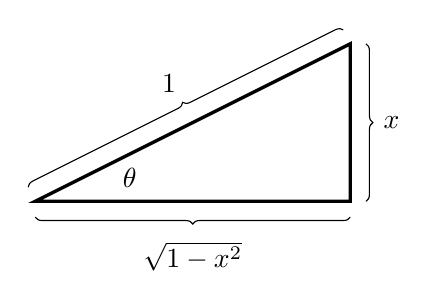
\begin{tikzpicture}
        \coordinate (C) at (0,2);
        \coordinate (D) at (4,2);
        \coordinate (E) at (4,4);
        \tkzMarkRightAngle(C,D,E)
        \tkzMarkAngle(D,C,E)
        \draw[decoration={brace,mirror,raise=.2cm},decorate,thin] (0,2)--(4,2);
        \draw[decoration={brace,mirror,raise=.2cm},decorate,thin] (4,2)--(4,4);
        \draw[decoration={brace,raise=.2cm},decorate,thin] (0,2)--(4,4);
        \draw[very thick] (D)--(E)--(C)--cycle;
        \node at (2,2-.7) {$\sqrt{1-x^2}$}; %% adj
        \node[anchor=west] at (4+.3,3) {$x$}; %% opp
        \node at (2-.3,3+.5) {$1$}; %% hyp
        \node at (1.2,2.3) {$\theta$};
      \end{tikzpicture}
    \end{image}
    Thus
    \begin{align*}
      \int \sqrt{1-x^2} \d x &= \frac{\theta}{2} +\frac{1}{2}\sin(\theta)\cos(\theta)+C \\
      &= \answer[given]{\frac{\arcsin(x)}{2} + \frac{x\sqrt{1-x^2}}{2}} + C 
    \end{align*}
  \end{explanation}
\end{example}

\begin{question}
  If
  \[
  \int \sqrt{1-x^2} \d x = \frac{\arcsin(x)}{2} + \frac{x\sqrt{1-x^2}}{2} + C,
  \]
  then
  \[
  \int_{-1}^{1}\sqrt{1-x^2} \d x = \answer{\pi/2}
  \]
\end{question}


Let's see a more complex example.


\begin{example}
  Compute:
  \[
  \int \frac{x^3}{x^2+9} \d x
  \]
  \begin{explanation}
    To start, recall the Pythagorean identity
    \[
    \tan^2(\theta) + 1 = \answer[given]{\sec^2(\theta)}
    \]
    and note that multiplying the entire equation by $9$ yields
    \[
    \left(\answer[given]{3\tan(\theta)}\right)^2 + 9 = (3\sec(\theta))^2.
    \]
    Hence we'll make the substitution
    \begin{align*}
      x &= 3\tan(\theta),\\
      \d x &= \answer[given]{3\sec^2(\theta)} \d \theta,
    \end{align*}
    Write with me
    \begin{align*}
      \int \frac{x^3}{x^2+9} \d x &= \int \frac{(3\tan(\theta))^3}{(3\tan(\theta))^2+9} \cdot 3\sec^2(\theta) \d \theta\\
      &=\int \frac{(3\tan(\theta))^3}{(3\sec(\theta))^2} \cdot 3\sec^2(\theta) \d \theta\\
      &=9\int \tan^3(\theta)  \d \theta.
    \end{align*}
    We'll use our expertise with trigonometric integrals
    \begin{align*}
      9\int \tan^3(\theta)  \d \theta &= 9\int \sin^3(\theta)\cos^{-3}(\theta)  \d \theta\\
      &= 9\int \sin^2(\theta)\cos^{-3}(\theta)  \sin(\theta) \d \theta\\
      &= 9\int (1-\cos^2(\theta))\cos^{-3}(\theta)  \sin(\theta) \d \theta
    \end{align*}
    Now set
    \begin{align*}
      g&=\cos(\theta),\\
      \d g &= \answer[given]{-\sin(\theta)}\d \theta,
    \end{align*}
    to find
    \begin{align*}
      &= -9\int \frac{1-g^2}{g^3}\d g\\
      &= -9\int g^{-3}-\frac{1}{g}\d g\\
      &= -9\left(\answer[given]{\frac{g^{-2}}{-2}}-\ln|g|\right) + C\\
      &= \frac{9}{2g^2} + 9\ln|g| + C.
    \end{align*}
    Now that we have an answer in $g$, we must convert it back to
    being a function in $\theta$, and then to a function in $x$. Write
    with me, since $g = \cos(\theta)$ we have
    \[
    \frac{9}{2g^2} + 9\ln|g| + C = \frac{9}{2\cos^2(\theta)} + 9\ln|\cos(\theta)| + C.
    \]
    To convert our answer to a function in $x$, use a reference
    triangle, noting that $3\tan(\theta) = x$, and so $\tan(\theta) =
    x/3$:
    \begin{image}
      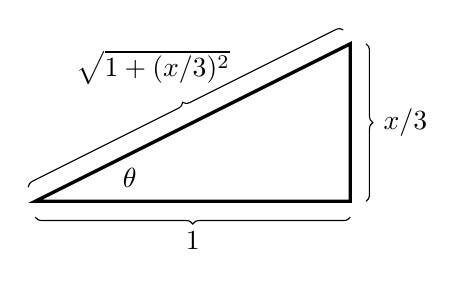
\begin{tikzpicture}
        \coordinate (C) at (0,2);
        \coordinate (D) at (4,2);
        \coordinate (E) at (4,4);
        \tkzMarkRightAngle(C,D,E)
        \tkzMarkAngle(D,C,E)
        \draw[decoration={brace,mirror,raise=.2cm},decorate,thin] (0,2)--(4,2);
        \draw[decoration={brace,mirror,raise=.2cm},decorate,thin] (4,2)--(4,4);
        \draw[decoration={brace,raise=.2cm},decorate,thin] (0,2)--(4,4);
        \draw[very thick] (D)--(E)--(C)--cycle;
        \node at (2,2-.5) {$1$}; %% adj
        \node[anchor=west] at (4+.3,3) {$x/3$}; %% opp
        \node at (2-.5,3+.7) {$\sqrt{1+(x/3)^2}$}; %% hyp
        \node at (1.2,2.3) {$\theta$};
      \end{tikzpicture}
    \end{image}
    Thus
    \[
    \cos(\theta) =  \answer[given]{\frac{1}{\sqrt{1+(x/3)^2}}}
    \]
    and we may write
    \begin{align*}
      \int \frac{x^3}{x^2+9} \d x &= \frac{9}{2\cos^2(\theta)} + 9\ln|\cos(\theta)| + C\\
      &= \frac{9+x^2}{2} + 9 \ln\left|\frac{1}{\sqrt{1+(x/3)^2}}\right| + C.
    \end{align*}
  \end{explanation}
\end{example}


However, sometimes the integral may not be in a form that is clear.
The key idea is to \dfn{complete the square}, and then choose a
trigonometric function which allows the use of a Pythagorean identity
to simplify the expression.



\begin{example}
  Compute:
  \[
  \int \frac{\sqrt{x^2+6x+5}}{x+3}\d x
  \]
  \begin{explanation}
    First we complete the square of the quadratic:
    \begin{align*}
      x^2+6x+5 &= x^2+6x+\answer[given]{9}+(5-\answer[given]{9})\\
      &= (\answer[given]{x+3})^2-4
    \end{align*}
    Our integral is now
    \[
    \int \frac{\sqrt{(x+3)^2-4}}{x+3}\d x
    \]
    We would like to choose to let $(x+3)$ equal some trigonometric
    function that will simplify after the application of a
    Pythagorean identity. Recall the Pythagorean identity
    \[
    \tan^2(\theta) + 1 = \sec^2(\theta)
    \]
    so we'll multiple this equation by $4$ and rearrange to find
    \[
    (\answer[given]{2\tan(\theta)})^2 = (\answer[given]{2\sec(\theta)})^2 - 4
    \]
    and set
    \begin{align*}
      (x+3) &=  2\sec(\theta)\\
      \d x &= 2\sec(\theta)\tan(\theta) \d \theta.
    \end{align*}
    So making this substitution we have
    \begin{align*}
      \int &\frac{\sqrt{(x+3)^2-4}}{x+3}\d x \\
      &= \int\frac{\sqrt{(\answer[given]{2\sec(\theta)})^2-4}}{\answer[given]{2\sec(\theta)}} \cdot 2\sec(\theta)\tan(\theta)\d \theta\\
      &= \int\frac{\sqrt{(2\tan(\theta))^2}}{2\sec(\theta)} \cdot 2\sec(\theta)\tan(\theta)\d \theta\\
    \end{align*}
    We will now assume $\tan(\theta)>0$ and leave the case when
    $\tan(\theta)<0$ to the intrepid young mathematician. Hence we may
    cancel the secants and simplify to:
    \[
    \int 2 \tan^2(\theta) \d \theta = 2\int \tan^2(\theta) \d \theta
    \]
    We'll again use the Pythagorean identity
    \[
    \tan^2(\theta) + 1 = \sec^2(\theta)
    \]
    to write
    \begin{align*}
      &= 2\int \sec^2(\theta) - 1 \d \theta\\
      &= \answer[given]{2\left(\tan(\theta) - \theta\right)} + C
    \end{align*}
    Now that we have an answer in $\theta$, we must convert it back to
    being a function in $x$. Write
    with me, since $x+3 = 2\sec(\theta)$ we have
    \[
    \cos(\theta) = \frac{2}{x+3},
    \]
    and using a reference triangle,
    \begin{image}
      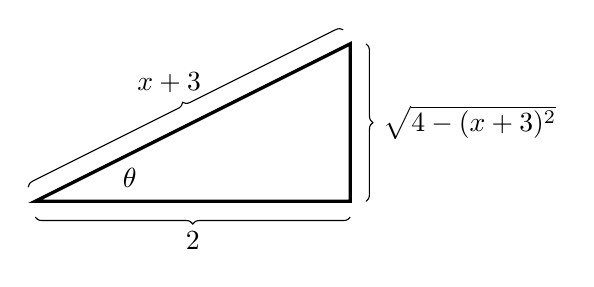
\begin{tikzpicture}
        \coordinate (C) at (0,2);
        \coordinate (D) at (4,2);
        \coordinate (E) at (4,4);
        \tkzMarkRightAngle(C,D,E)
        \tkzMarkAngle(D,C,E)
        \draw[decoration={brace,mirror,raise=.2cm},decorate,thin] (0,2)--(4,2);
        \draw[decoration={brace,mirror,raise=.2cm},decorate,thin] (4,2)--(4,4);
        \draw[decoration={brace,raise=.2cm},decorate,thin] (0,2)--(4,4);
        \draw[very thick] (D)--(E)--(C)--cycle;
        \node at (2,2-.5) {$2$}; %% adj
        \node[anchor=west] at (4+.3,3) {$\sqrt{4-(x+3)^2}$}; %% opp
        \node at (2-.3,3+.5) {$x+3$}; %% hyp
        \node at (1.2,2.3) {$\theta$};
      \end{tikzpicture}
    \end{image}
    Thus
    \[
    \tan(\theta) = \answer[given]{\frac{\sqrt{4-(x+3)^2}}{2}}
    \]
    and we may write
    \begin{align*}
    \int &\frac{\sqrt{(x+3)^2-4}}{x+3} \d x = 2\left(\tan(\theta) - \theta\right) + C\\
      &= \sqrt{4-(x+3)^2} - 2\arctan\left(\frac{\sqrt{4-(x+3)^2}}{2}\right) + C.
    \end{align*}
  \end{explanation}
\end{example}


\section{Summary}

In general:
\begin{itemize}
\item If the quadratic has the form $a^2 + x^2$ after completing the square, make the substitution $u = a\tan(\theta)$
\item If the quadratic has the form $a^2 - x^2$ after completing the square, make the substitution $u = a\sin(\theta)$ 
\item If the quadratic has the form $x^2 - a^2$ after completing the
  square, make the substitution $u = a\sec(\theta)$
\end{itemize}
The choices $a\cot(\theta)$, $a\cos(\theta)$, and $a \csc(\theta)$
could be used with equal efficiency, but there is no reason to ever
use them.


\end{document}
